\subsection{Wizualizacja}
Wizualizacja modeli 3D stanowi wyzwanie dla użytkownika końcowego,
głównie z powodu braku spójnych platform umożliwiających realizację
całego procesu – od wgrania plików wejściowych po interakcję z modelem – w ramach jednej aplikacji.
Dostępne na rynku rozwiązania wymagają korzystania z aplikacji trzecich i pewnej wiedzy technicznej,
co prowadzi do problemów z integracją i spójnością działania.

Celem projektu było stworzenie intuicyjnego, dynamicznego i responsywnego \textbf{interfejsu} zintegrowanego z wydajnym \textbf{renderingiem} GPU.
Aplikacja umożliwia użytkownikowi końcowemu realizację pełnego procesu
wizualizacji – od tworzenia i modyfikacji modelu po jego segmentację i wyświetlanie – w jednej aplikacji.
Projekt rozwiązuje problem fragmentarycznej funkcjonalności dostępnych aplikacji, oferując spójne środowisko do obsługi modeli 3D.

\textbf{Korzyści z realizacji projektu}

\begin{itemize}
    \item zwiększoną wydajność dzięki GPU,
    \item eliminację konieczności korzystania z wielu narzędzi,
    \item uproszczony proces użytkowania, co zwiększa dostępność aplikacji dla mniej zaawansowanych użytkowników.
\end{itemize}

Rendering wykorzystuje plik .ply jako dane wejściowe do wczytania splatów.
Są one renderowane jako sześciany, w których wnętrzu generowane są shadery, bazujące na skalowaniu i rotacji splatów.
Takie podejście umożliwia abstrakcyjne przedstawienie splatów przy jednoczesnym zachowaniu wysokiej dokładności wizualnej.

Interfejs został zaimplementowany w:
\begin{itemize}
    \item QML
    \item PyQt
\end{itemize}

Rendering został zaimplementowany w:
\begin{itemize}
    \item C
    \item OpenGL
    \item OpenCL
\end{itemize}

\begin{figure}[h!]
    \centering
    \begin{minipage}{0.245\textwidth}
        \centering
        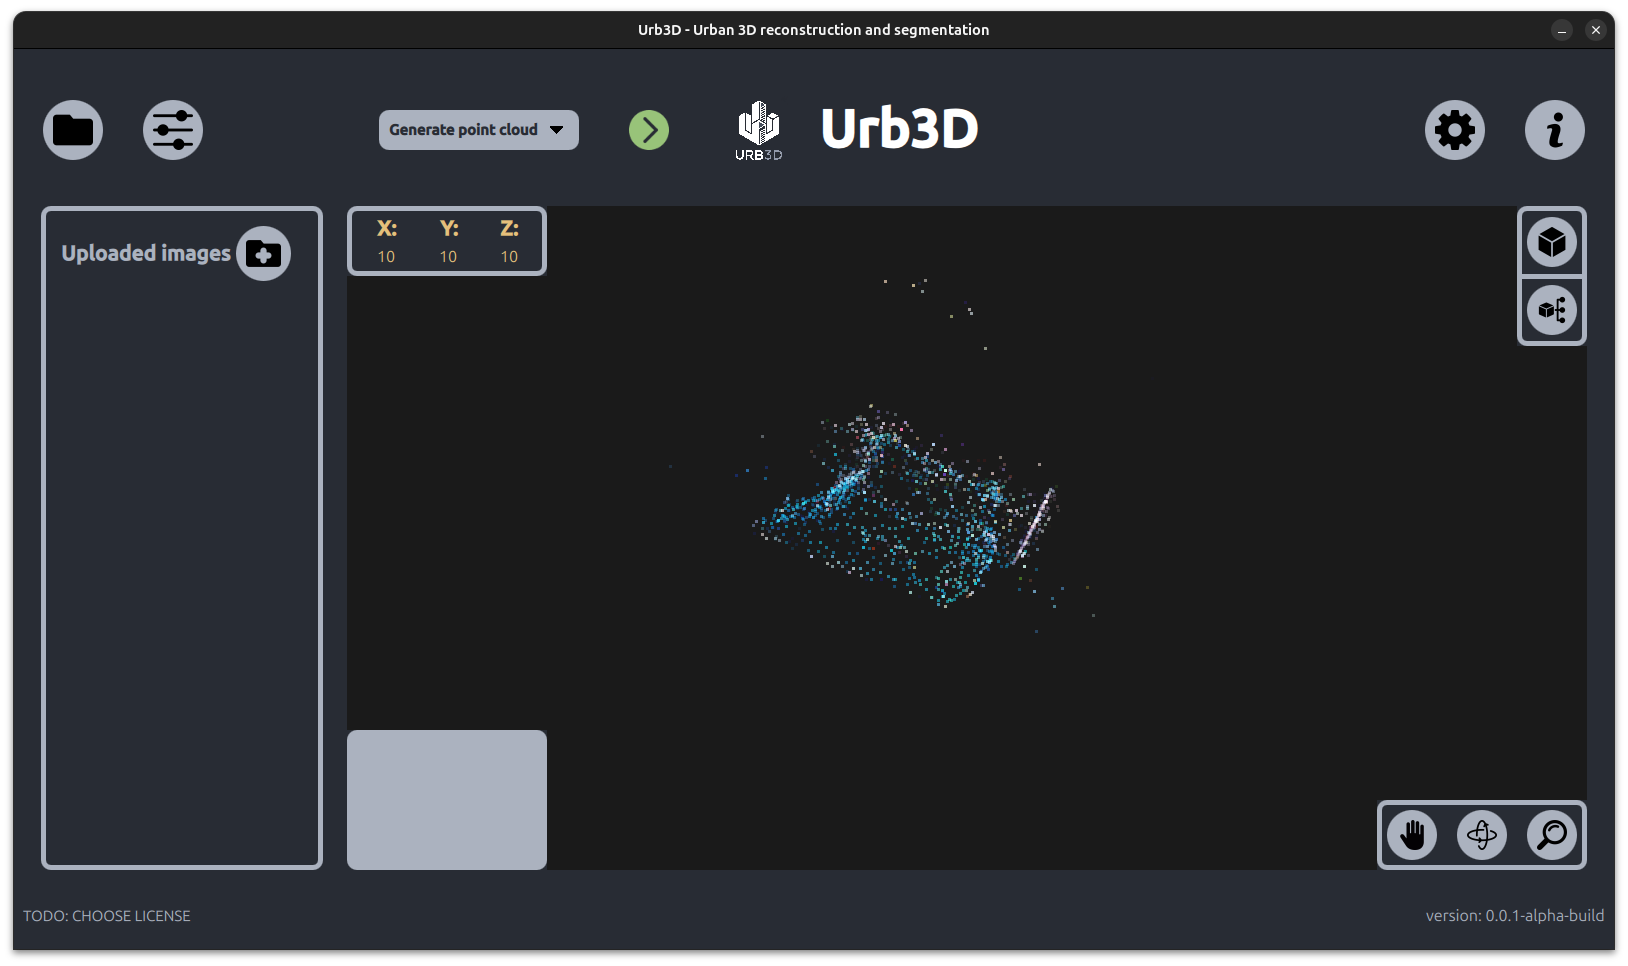
\includegraphics[width=\textwidth]{images/UI-Rendering.png}
    \end{minipage}
    \caption{Zrzut ekranu przedstawiający główny widok aplikacji}
    \label{fig:ui-rendering}
\end{figure}

\begin{figure}[h!]
    \centering
    \begin{minipage}{0.245\textwidth}
        \centering
        \includegraphics[width=\textwidth]{} % DODAM JESZCZE
    \end{minipage}
    \caption{Zrzut ekranu przedstawiający własny renderer}
    \label{fig:rendering}
\end{figure}